\subsection{Energy Harvesting Systems}
\label{sec:background_harvesting}

Energy harvesting devices operate using energy extracted from sources such as
radio frequency transmissions and solar energy. These devices elide tethered
power or a battery, instead collecting energy into a capacitor, operating when
sufficient energy accumulates, and upon depleting the energy, turning off and
recharging.
There are several energy harvesting battery-less hardware platforms. For
instance, computational RFIDs---open-source TI MSP430-based~\cite{wolverine}
WISP~\cite{wisp5} (with its variants such as
WISPCam~\cite{naderiparizi_rfid_2015}, NFC-WISP~\cite{zhao_rfid_2015} or
NeuralWISP~\cite{holleman_biocas_2008}), Moo~\cite{moo}, and commercial ones
such as~\cite{medusa_farsens_2017}. Other platforms include ambient backscatter
tag~\cite{liu_sigcomm_2013,parks_sigcomm_2014} or battery-less
phone~\cite{talla_imwut_2017}. 

\textbf{Hardware Assumptions.} \sys is designed for the demands of existing and
future energy-harvesting platforms based around general purpose, commodity
computing components~\cite{wisp,msp430datasheet}. We assume a device with a
memory system that has fast, byte-addressable volatile and non-volatile memory;
in particular, our target platform, WISP~\cite{wisp}, is equipped with a
mixture of SRAM and FRAM. Our implementation leverages hardware support for
fast, bulk-copying between memories via DMA~\cite{msp430datasheet}. \sys does not
require architectural additions to commodity processors as
in~\cite{su_date_2017,hicks_isca_2017,quickrecall,nvp}.

\subsection{Intermittent Execution}
\label{sec:background_consistency}

\begin{figure}
    \begin{subfigure}{0.49\columnwidth}
        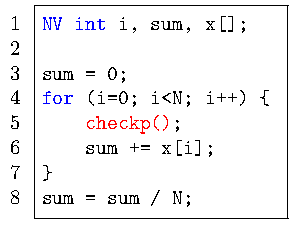
\includegraphics[width=\columnwidth]{figures/war-example.pdf}
        \caption{Subcaption}
        \label{fig:war-example}
    \end{subfigure}
    \begin{subfigure}{0.49\columnwidth}
        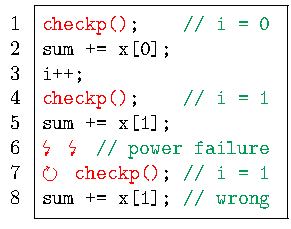
\includegraphics[width=\columnwidth]{figures/war-execution.pdf}
        \caption{Subcaption}
        \label{fig:war-execution}
    \end{subfigure}
    \caption{Main caption.}
    \label{fig:war}
\end{figure}

Software running on an energy-harvesting device executes {\em intermittently}
because energy sources are not always available to harvest and buffer
sufficient operational energy. An intermittent execution is composed of
operating periods interspersed with power
failures~\cite{dino,chain,alpaca,ratchet}. The frequency of failures depends on
the size of the device's energy storage buffer: a larger buffer allows longer
operating periods. 

A power failure clears volatile state (e.g., registers and SRAM) while
non-volatile memory (e.g., FRAM) persists. Upon a power failure, control flows
to a prior point in the execution: by default, to the beginning of {\tt
main()}. Early intermittent systems preserved progress by periodically
checkpointing volatile execution context to non-volatile
memory~\cite{mementos}, sometimes using hardware
support~\cite{mottola2017harvos,hibernusplusplus,hibernus,idetic,quickrecall}. 

Checkpointing volatile state alone do not ensure data consistency when the
system can directly manipulate non-volatile memory~\cite{mspcdino}.
Especially, data can get inconsistent when code includes a
\emph{write-after-read} (WAR) dependence between operations that manipulate
non-volatile memory, because it allows {\em writes} from a failed attempt to
persist across failure and be read by the {\em
reads}~\cite{ratchet,dino,alpaca}\TODO{figure 2 dependent text ---see
Figure~\ref{fig:code_demo_incosistency} that illustrates how state can become
inconsistent in an intermittent execution using the cyclic redundancy check
(CRC) code from MIBench2~\cite{hicks_mibench2_2016}.  Additional method to
maintain data consistent in the presence of WAR dependency is necessary for
correct execution.}


\subsection{Task-based Intermittent Programming}
\label{section:background_task_computing}

Task-based execution models~\cite{dino,chain,alpaca} ask the programmer to
decompose their program into \textbf{tasks}, which is a region of code that can contain
arbitrary computation, sensing, and communication.  Task-based models progress at the granularity of tasks. They re-execute each task interrupted by a power failure until it successfully finishes, only then moving on to
the next task. Since these models do not rely on taking an expensive
checkpoint, they are usually faster than the checkpoint-based
solution~\cite{chain, alpaca}.  \sys also follows the paradigm of the
task-based programming model, where the programmer explicitly expresses the
application as a sequence of tasks and the transitions between them.

Task-based models also suffer from data inconsistency when there is a WAR
dependence.  Prior systems tried to tackle the problem by a compiler-automated
redo-logging for the variables that is part of the dependence~\cite{alpaca}, or
by statically creating multiple copies of the problematic variable to ensure
that no task reads and writes the same copy~\cite{chain}.

\subsection{Costs of Previous Models}
\label{sec:cost_task-based}

Prior systems, including the task-based models, suffer from two major overheads:
{\em frequent non-volatile memory access} and {\em incorrectly sized, inefficient or non-terminating tasks}.

\begin{table}
	\centering
	\footnotesize
	\begin{tabular}{|c|c|}
		\hline
		Model & Data Copied to/from NVRAM \\
		\hline\hline
		Mementos~\cite{mementos}	& Registers + Stack     \\
		DINO~\cite{dino}	& Registers + Stack + WAR NV variables \\%used in task\\
		Chain~\cite{chain}	& PC + NV variables used in task\\
		Alpaca~\cite{alpaca}	& PC + WAR NV variables used in task\\
		Ratchet~\cite{ratchet}, Clank~\cite{hicks_isca_2017} & Registers (requires NV main memory) \\
		Region Formation~\cite{baghsorkhi_cgo_2018} & Registers + Updated variables in task \\
		\hline
	\end{tabular}
	\caption{Non-volatile memory access for data consistency; \emph{PC}: program counter, \emph{WAR variables}: variables involved in Write after Read (WAR) dependences, \emph{NV}: non-volatile.}
	\label{table:chechpoint_comparison}
\end{table}


\textbf{Frequent Non-volatile Memory Access.} 
Previous systems frequently access the non-volatile memory directly, which is a potential source of inefficiency.  Checkpointing systems copy all volatile
state~\cite{dino, mementos, ratchet, hicks_isca_2017} to non-volatile memory at
every checkpoint.  Task-based models, which do not take checkpoints, back up a
subset of non-volatile data to maintain memory consistency using, e.g.,
redo-logging.  Table~\ref{table:chechpoint_comparison} summarizes the data that
gets copied to and from the non-volatile memory in service of memory
consistency and progress preservation.  Ratchet~\cite{ratchet} and
Clank~\cite{hicks_isca_2017}, which require all memory to be non-volatile
perform high-frequency non-volatile memory accesses, into checkpointing
frequently.

\textbf{Incorrectly Sized Tasks Problem.} Compiler-inserted checkpoints or
programmer-defined tasks can be both non-terminating and/or
inefficient.  If a task (or code between two checkpoints) consumes more than the fixed,
maximum energy that the device can buffer, then the task
will never be able to complete using buffered energy.  Such a task is
non-terminating, {\em prevents forward progress}, and makes the program
incorrect. 
%
If the task consumes far less energy than a device can buffer, the system
may operate {\em inefficiently}, saving the program state more often than needed.
%
Avoiding excessively costly, non-terminating, tasks and short, high-overhead,
tasks is challenging, because estimating the exact energy use of an arbitrary code is complicated.  
Moreover, when \emph{heterogeneous devices} with different energy buffers (e.g., 20\,$\mu $F~\cite{rodriguez_tbcs_2015} to 0.1\,F~\cite{moo}) are considered the problem of porting a program become much worse
because a large task on one device may be a relatively short task
on a device with a larger buffer.
%
\textbf{\sys's execution model} solves this dilemma by introducing {\em task coalescing}, which
merges multiple tasks to amortize the overhead when tasks are too small, and
{\em task downscaling}, which breaks up a task when the task is too large to complete. 
